\documentclass[11pt]{article}
\usepackage[margin=0.82in]{geometry}
\usepackage{amsmath,amssymb}
\usepackage{booktabs}
\usepackage{graphicx}
\usepackage{xcolor}
\usepackage[hidelinks]{hyperref}

\definecolor{warning}{RGB}{145,75,0}

\title{Why the $F_{30}$ Periodic Brake Candidate Nearly Reaches\\
the Rational $3{:}4{:}5$ Burrau Initial Condition}
\author{}
\date{September 5, 2026}

\begin{document}
\maketitle

\noindent
\textbf{Evidence status.}
The orbit discussed here is an ordinary high-precision numerical shooting
solution, supported by independent integrations and a global Levi--Civita
coordinate calculation.  A validated interval proof that the exact periodic
root exists has not yet been completed.  It is therefore a very strong
numerical candidate, not a theorem or a Pythagorean counterexample.

\section*{1. The exact rational target}

Normalize the longest side and its opposite mass to one.  The $3{:}4{:}5$
Burrau initial condition is
\[
 (m_1,m_2,m_3)=\left(\frac35,\frac45,1\right)
                 =(0.6,0.8,1),
\]
\[
 q_1=\left(-\frac12,0\right),\qquad
 q_2=\left( \frac12,0\right),\qquad
 q_3=\left(\frac{7}{50},\frac{12}{25}\right)=(0.14,0.48),
\]
with all three velocities zero.  Every number in these normalized launch data
is rational.  The opposite side lengths are exactly $3/5$, $4/5$, and $1$,
and
\[
 \left(\frac35\right)^2+\left(\frac45\right)^2=1.
\]
In the Euclid parameterization this point is $u=1/2$, or $u=1/3$ after
exchanging the legs.

\section*{2. Where $F_{30}$ came from}

Li and Liao searched for free-fall periodic brake orbits while holding the
masses fixed at the exact rational ratio $(0.6,0.8,1)$ and allowing the
initial triangle to vary.  One catalog orbit, $F_{30}$, began at
\[
 q_3\simeq(0.1446319096,0.4773197126),
\]
only about $5.35\times10^{-3}$ from the exact $3{:}4{:}5$ launch vertex.
Thus the first reason for the proximity is deliberate selection: the parent
catalog slice already had the exact $3{:}4{:}5$ masses, and $F_{30}$ was the
catalog member whose brake triangle lay nearest the mass--side-tied target.

We then varied the two independent mass ratios and solved five equations:
three equations demanding a simultaneous second brake and two equations
demanding that each varied mass equal its opposite initial side.  The nearby
shooting root is
\[
 (m_1,m_2,m_3)\simeq
 (0.594811646571005,\;0.801774973317793,\;1),
\]
\[
 q_3\simeq(0.144521106471,\;0.476902140016),
 \qquad \tau\simeq6.28923382379.
\]
Doubling the brake-to-brake segment gives the numerically periodic labelled
orbit shown below.

\begin{figure}[ht]
  \centering
  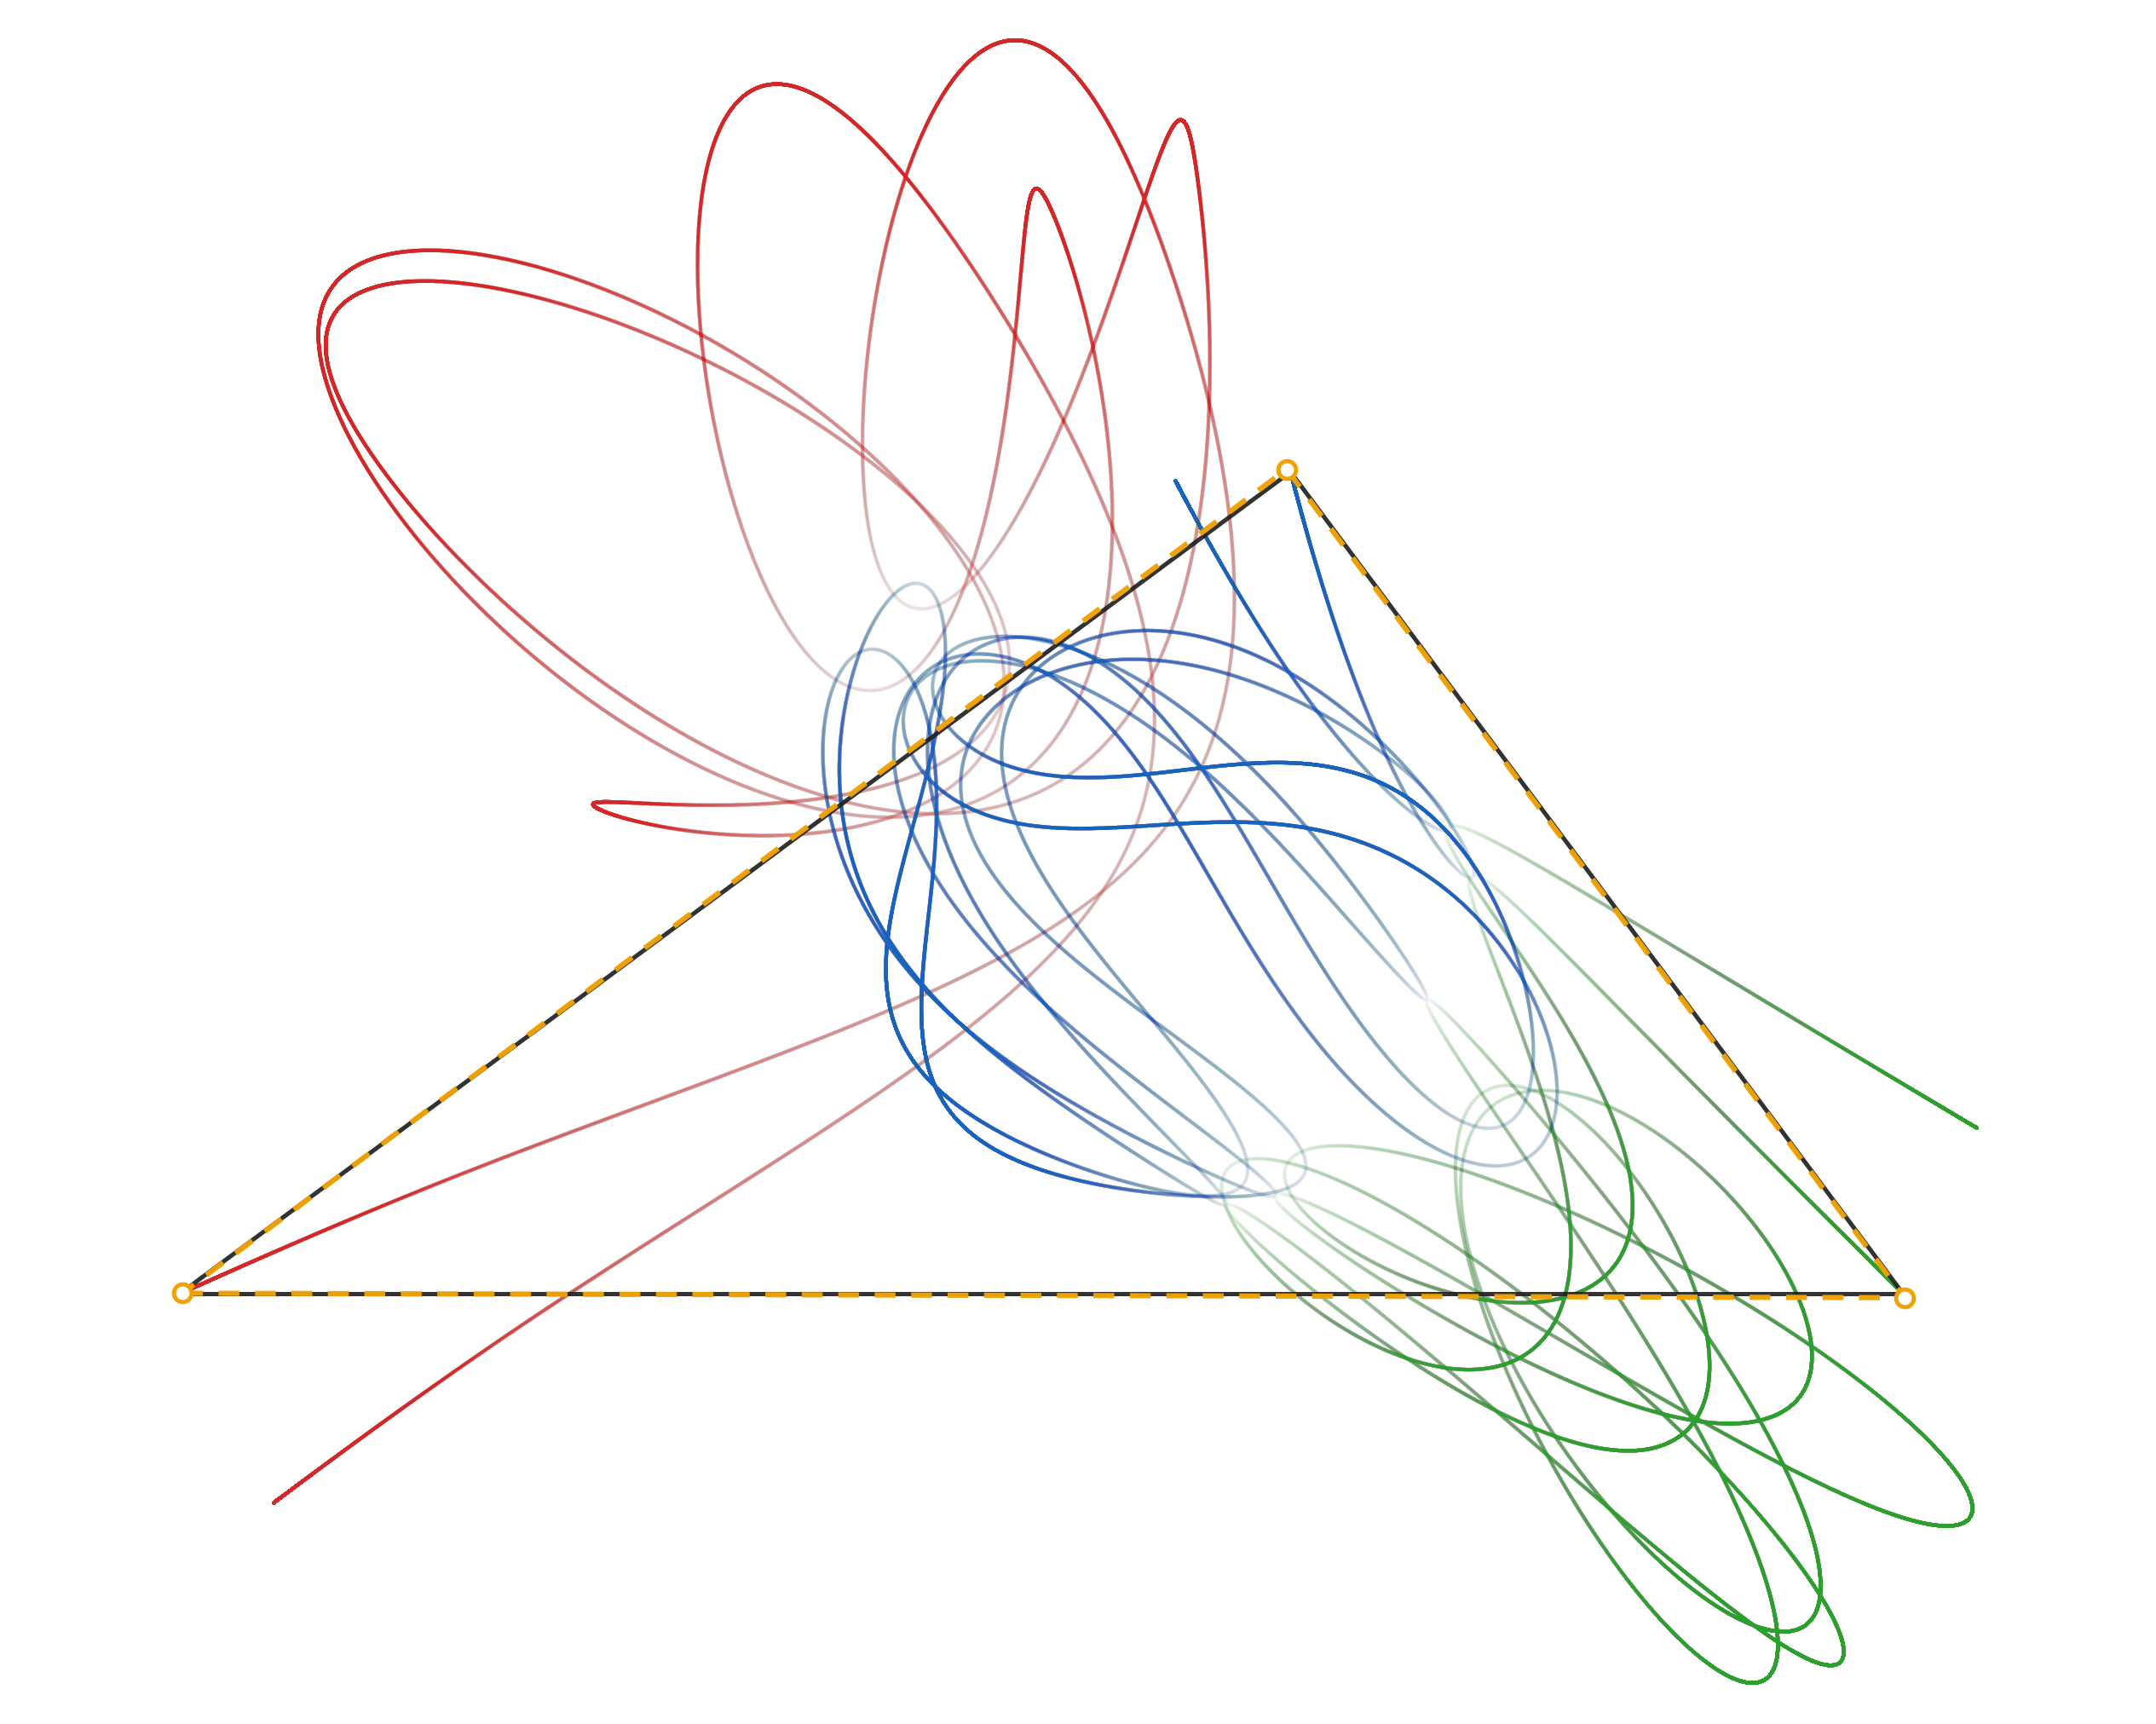
\includegraphics[width=0.92\linewidth]{../plots/f30_mass_side_periodic_candidate.png}
  \caption{The $F_{30}$ mass--side periodic candidate.  Red, green, and blue
  trace the three labelled bodies at uniform increments of physical time.
  The solid dark triangle is the actual initial condition.  The dashed gold
  triangle is the labelled $3{:}4{:}5$ triangle after optimal translation,
  rotation, and one common scaling.}
\end{figure}

\section*{3. How close is it?}

\begin{center}
\begin{tabular}{@{}lrrr@{}}
\toprule
Quantity & Exact $3{:}4{:}5$ & $F_{30}$ tied candidate & Difference \\
\midrule
$m_1$ & $0.600000000000$ & $0.594811646571$ & $-0.005188353429$ \\
$m_2$ & $0.800000000000$ & $0.801774973318$ & $+0.001774973318$ \\
$q_{3x}$ & $0.140000000000$ & $0.144521106471$ & $+0.004521106471$ \\
$q_{3y}$ & $0.480000000000$ & $0.476902140016$ & $-0.003097859984$ \\
$m_1^2+m_2^2-1$ & $0$ & $-0.003355997265$ & $-0.003355997265$ \\
largest initial angle & $90^\circ$ & $90.2015966^\circ$ & $+0.2015966^\circ$ \\
\bottomrule
\end{tabular}
\end{center}

The two leg masses differ from $3/5$ and $4/5$ by approximately $-0.865\%$
and $+0.222\%$.  The candidate's leg-vector length is
\[
 \sqrt{m_1^2+m_2^2}\simeq0.9983205912,
\]
so the unit side is only about $0.168\%$ longer than the hypotenuse that would
make these particular two legs exactly right.

For the figure, let $z_i$ be the complex vertices of the exact labelled
$3{:}4{:}5$ triangle and $w_i$ the actual launch vertices.  The displayed
reference minimizes
\[
 \sum_{i=1}^3\left|w_i-\bigl(b+\alpha(z_i-\bar z)\bigr)\right|^2
\]
over the translation $b$ and the complex multiplier $\alpha$, which supplies
one rotation and one positive common scale but no reflection or relabeling.
The optimal scale is
\[
 |\alpha|\simeq0.9991493750,
\]
and the RMS vertex mismatch after alignment is only
\[
 2.23745\times10^{-3}.
\]

\section*{4. Why a small continuation was enough}

Away from collision, a nondegenerate periodic shooting root varies smoothly
when the masses vary.  The original $F_{30}$ triangle already nearly satisfied
the two mass--side equations.  Allowing both independent mass ratios to move
therefore supplied exactly two controls with which to drive those two side
residuals to zero while the three second-brake equations were maintained.

The orbit also has a long sequence of syzygies and an extremely close binary
passage, with a resolved separation of order $5\times10^{-4}$.  Such passages
make the return map highly sensitive: small changes in the launch geometry or
masses can produce large endpoint changes.  This helps explain why modest
parameter adjustments can repair several shooting residuals.  It is a
dynamical interpretation, however, not a theorem that forces an intersection
with the right-triangle locus.

The resulting mass--side solution appears locally isolated and transverse.
After the three brake equations and two mass--side equations have been imposed,
the right-angle equation
\[
 m_1^2+m_2^2=1
\]
is one additional condition with no remaining continuous tuning parameter.
No known symmetry forces it.  This is why the orbit gets remarkably close but
then stops at a defect of approximately $-0.003356$.

\section*{5. Is the $F_{30}$ initial condition rational?}

\begin{center}
\fcolorbox{warning}{white}{\parbox{0.88\linewidth}{
\textbf{No rationality result is known for the continued $F_{30}$ root.}
Its printed masses and coordinates are numerical approximations to a shooting
root.  Finite decimal approximations can prove neither rationality nor
irrationality.}}
\end{center}

There are three different statements that should not be conflated:
\begin{enumerate}
  \item The \emph{parent mass slice} $(3/5,4/5,1)$ is exactly rational.
  \item The original catalog orbit on that slice has numerical launch
        coordinates; those coordinates are not known to be rational.
  \item The continued mass--side candidate has numerical masses
        $(0.594811\ldots,0.801775\ldots,1)$ and numerical coordinates.  They
        are not known to be rational or irrational.
\end{enumerate}

Moreover, the continued candidate is certainly not an exact Pythagorean
initial condition at the level of the computed root: its triangle is obtuse,
not right.  Even proving that one or both of its masses were rational would not
repair the nonzero Pythagorean defect.

One may project the candidate's mass pair radially onto the unit Pythagorean
circle.  Its angular direction then corresponds to
\[
 u_{\rm proj}=\frac{m_2}{\sqrt{m_1^2+m_2^2}+m_1}
              \simeq0.5032695682,
\]
near the rational value $1/2$.  But this is only a quantitative description
of proximity: because the unprojected candidate is not on the unit circle,
it has no actual Euclid parameter $u$.

\section*{Conclusion}

$F_{30}$ is close to a rational Pythagorean initial condition for two concrete
reasons: it was selected from the exact rational $3{:}4{:}5$ mass slice, and a
smooth two-mass continuation then imposed the two mass--side constraints with
only a small displacement.  Its complicated close-encounter dynamics gives
the shooting map enough sensitivity to make this adjustment possible.  What
is still absent is an exact mechanism forcing the sixth condition---the right
angle---or forcing the resulting root to have rational arithmetic data.

\end{document}
